\documentclass[simplex.tex]{subfiles}
% NO NEED TO INPUT PREAMBLES HERE
% packages are inherited; you can compile this on its own

\onlyinsubfile{
\title{NeuroData SIMPLEX Report: Subfile}
}

\begin{document}
\onlyinsubfile{
\maketitle
\thispagestyle{empty}

The following report documents the progress made by the labs of Randal~Burns and Joshua~T.~Vogelstein at Johns Hopkins University towards goals set by the DARPA SIMPLEX grant.

%%%% Table of Contents
\tableofcontents

%%%% Publications
\bibliographystyle{IEEEtran}
\begin{spacing}{0.5}
\section*{Publications, Presentations, and Talks}
%\vspace{-20pt}
\nocite{*}
{\footnotesize	\bibliography{simplex}}
\end{spacing}
%%%% End Publications
}

\subsection{Discriminability}

We develop a measure of discriminability (or reliability).  It
is intuitive to understand and easy to implement.
Discriminability is defined to be the probability of within
subject distances being smaller than the cross subject
distances. If we let $x_{i,t}$ denote the t$^{\text{th}}$ trial of subject 
$i$ and $\Delta(,)$ be the metric, the (population) discriminability $D$
is: $D= P (\Delta(x_{i,t} , x_{i,t’}) \leq  \Delta(x_{i,t} , x_{i’,t’’}))$.
We want to
search for the optimal processing pipeline which has the
maximal discriminability. Previously, we process 13 fMRI data
sets with 64 pipelines, and show some pipelines yields data
sets with high sample discriminability. Currently, we are
developing a statistical test to determine whether one
pipeline is significant better than the other. To develop a
valid test, we need to approximate the distribution of
difference between sample discriminability estimates under the
null hypothesis that two population discriminability are
equal. We design and implement a bootstrap procedure to
achieve this  which is described below.



\begin{figure}[h!]
\begin{cframed}
\centering
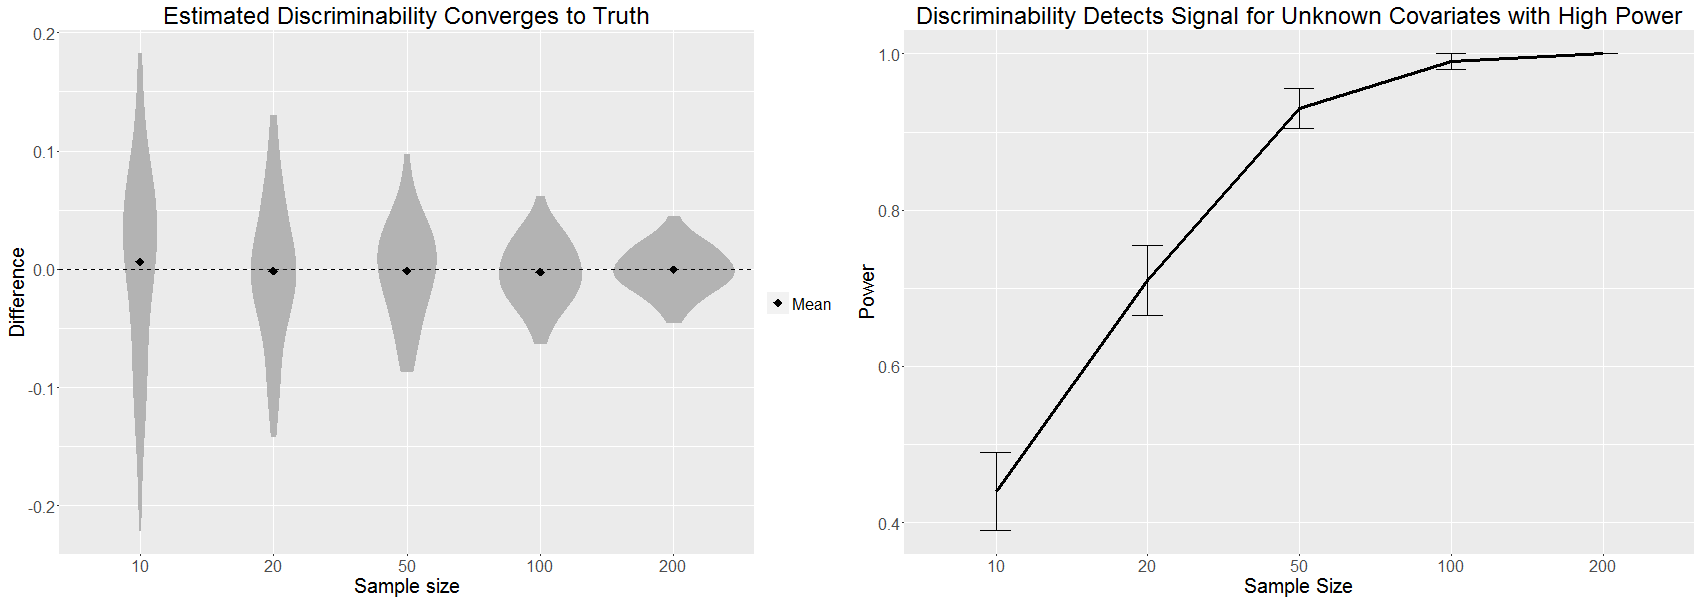
\includegraphics[width=0.75\textwidth]{./figs/discriminability1.png}
\caption{
{\bf Convergence of $\hat D$}
Distribution of difference between
discriminability estimates and truth is
shown in the left panel. The physical
property and noise are generated from
standard Gaussian distribution. The black
dots indicate the mean over 100 repeats. As
the number of subjects increases, the
sample discriminability converges to the
true population discriminability.  {\bf
Discriminability Test Power.} Test power
of discriminability with varying sample
size is shown in the right panel. The
physical property and noise are generated
from standard Gaussian distribution as
described in the simulation section. At
level of 0.05, the power is estimated based
on  100 repeats. The test power becomes close
to 1 with more than 50 samples.}
\label{fig:dis1}
\end{cframed}
\end{figure}

{\bf Testing the null hypothesis $D(\Psi_1) = D(\Psi_2)$}
Input: Data set, Pipeline $\Psi_1$, Pipeline $\Psi_2$
Output: Reject or do not reject the null hypothesis


\begin{compactenum}
\item Process the data set with pipelines $\Psi_1$ and $\Psi_2$
\item Compute $\hat D(\Psi_1)$ and $\hat D(d)$  
\item For \{$i$ in 1 through number of repeats\} 
  \begin{compactenum}
  \item For \{$j$ in 1 through number of subjects\} 
    \begin{compactenum}
    \item Randomly select two subjects from data set 
    \item Linearly combine measurements of these subjects
    \end{compactenum}
  \end{compactenum}
\item EndFor
\item Compute pairwise differences $D^{(i)}(\Psi_1) - D^{(i’)}(\Psi_1)$ and $D^{(i)}(\Psi_2) - D^{(i’)}(\Psi_2)$
\item Compute p-value which is the fraction of times that $\hat D(\Psi_1)−\hat D(\Psi_2) > D^{(i)}(\Psi_j) − D^{(i‘)}(\Psi_j)$
\item Reject the null hypothesis if $p$-value is less than 0.05.
\end{compactenum}


We are currently running the test procedure on 13 data sets
processed 64 ways. After finish running, we will have 13 p-values
for each pipeline. We will use Fisher’s method to combine
results.  


Furthermore, we take the previously computed fMRI
discriminability data and compare all pipelines to the CFXXG
pipeline (CC200 atlas, FSL, No Scrubbing, No Filtering, Signal
Regression) use Wilcoxon signed rank test. CFXSG pipeline has the
best mean discriminability across data sets. The result is shown
in figure \ref{fig:pipes}.


\begin{figure}[h!]
\begin{cframed}
\centering
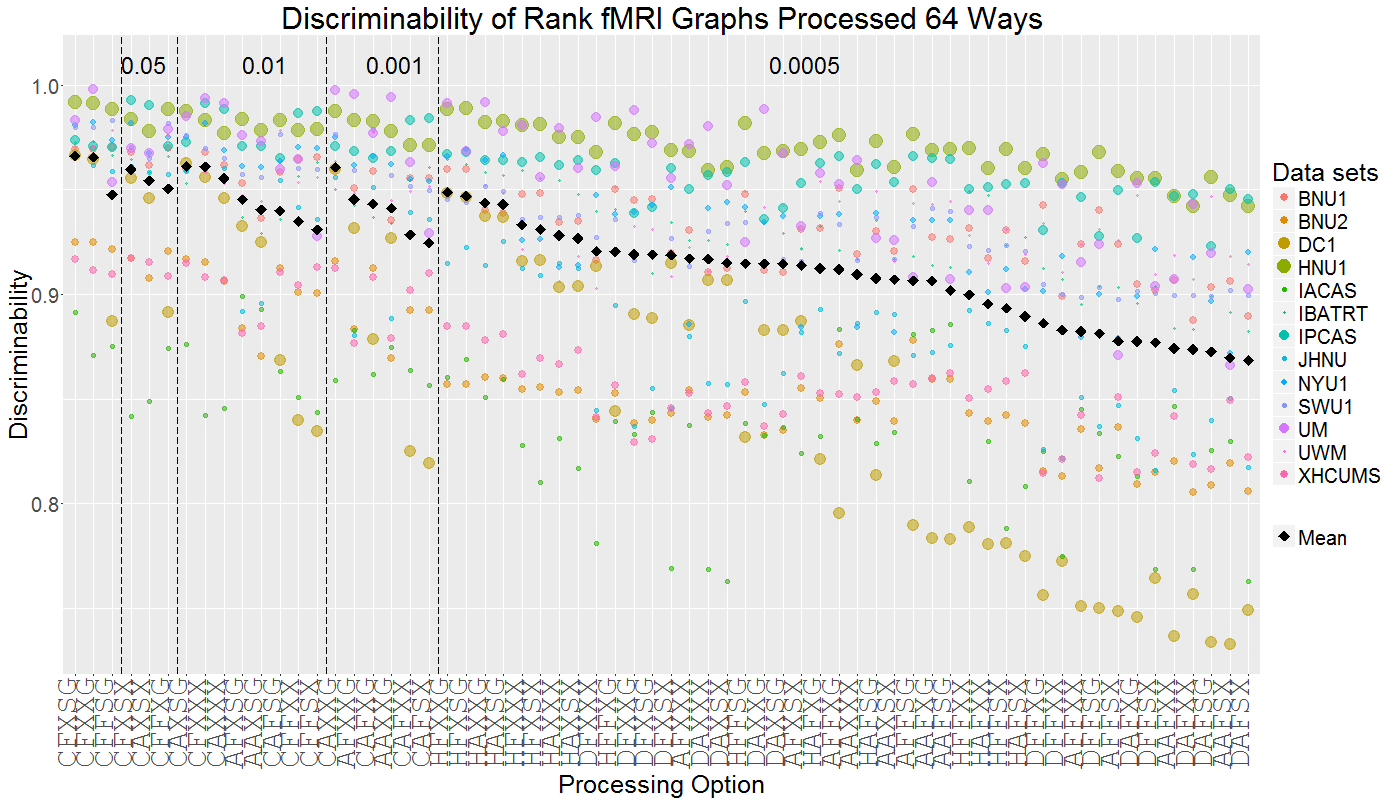
\includegraphics[width=\textwidth]{./figs/pipes.png}
\caption{
{\bf Discriminability of rank fmri graphs from 13 data sets processed 64 ways.}  Discriminability of BNU1, BNU2, DC1,HNU1, IACAS, IBATRT, IPCAS, JHNU, NYU1, SWU1, UM, UWM and XHCUMS pre-processed by 64 pipelines are computed and shown in the top panel. Color of each dot indicates data set and size indicates the number of measurements in data set. The black square indicates the weighted mean discriminability across 13 data sets. The pipelines are first grouped by p-values when comparing to pipeline CFXXG using Wilcoxon signed-rank test. The number at the top indicates the p-value when compared to CFXXG. Within each group, the pipelines are ordered by the mean discriminability. CFXSG pipeline has the best mean discriminability across data sets.}
\label{fig:pipes}
\end{cframed}
\end{figure}



\end{document}
